\documentclass[12pt]{article}
\usepackage{graphicx}
\usepackage{geometry}
\usepackage{hyperref}
\usepackage{listings}
\usepackage{xcolor}
\usepackage{titlesec}
\usepackage{float}
\usepackage{caption}
\geometry{margin=1in}

\title{E-Commerce Analytics on AWS RDS with Flask and FastAPI}
\author{[Your Full Name] \\ DevOps & Cloud Engineering Student}
\date{\today}

\definecolor{codegray}{rgb}{0.5,0.5,0.5}
\definecolor{codepurple}{rgb}{0.58,0,0.82}
\definecolor{backcolour}{rgb}{0.95,0.95,0.92}
\lstdefinestyle{mystyle}{
    backgroundcolor=\color{backcolour},   
    commentstyle=\color{codegray},
    keywordstyle=\color{blue},
    numberstyle=\tiny\color{codegray},
    stringstyle=\color{codepurple},
    basicstyle=\ttfamily\footnotesize,
    breaklines=true,
    frame=single,
    numbers=left,
    numbersep=5pt,
    showstringspaces=false
}
\lstset{style=mystyle}

\begin{document}
\maketitle
\tableofcontents
\newpage

\section{Introduction}
This project demonstrates the creation of an e-commerce analytics system using AWS RDS for MySQL and Python-based APIs. It includes database modeling, SQL analytics, API design using Flask and FastAPI, and API testing with Postman.

\section{Database Setup on AWS RDS}
\subsection{Steps}
\begin{enumerate}
    \item Launched an AWS RDS MySQL instance (version 8.0).
    \item Enabled public access and set port 3306 open to current IP.
    \item Connected using MySQL Workbench for schema creation and data insertion.
\end{enumerate}

\section{SQL Schema and Data Insertion}
The database contains 4 main tables: \texttt{customers}, \texttt{products}, \texttt{orders}, and \texttt{order\_items}. Below is the schema setup.

\subsection{Schema Creation}
\begin{lstlisting}[language=SQL, caption=Database Schema Script]
DROP TABLE IF EXISTS order_items;
DROP TABLE IF EXISTS orders;
DROP TABLE IF EXISTS products;
DROP TABLE IF EXISTS customers;

CREATE TABLE customers (
 customer_id INT PRIMARY KEY,
 name VARCHAR(100),
 email VARCHAR(100) UNIQUE,
 country VARCHAR(50)
);
-- Products, Orders, Order Items follow...
\end{lstlisting}

\subsection{Data Insertion}
\begin{lstlisting}[language=SQL, caption=Sample Data Insert]
INSERT INTO customers VALUES
(1, 'Alice Smith', 'alice@example.com', 'USA'),
(2, 'Bob Jones', 'bob@example.com', 'Canada'),
(3, 'Charlie Zhang', 'charlie@example.com', 'UK');
-- Products, Orders, and Order Items follow...
\end{lstlisting}

\section{Analytical Queries}
Each SQL query below extracts useful business insights from the data.

\subsection{Top Customers by Spending}
\begin{lstlisting}[language=SQL]
SELECT c.name, SUM(oi.quantity * oi.unit_price) AS total_spent
FROM customers c
JOIN orders o ON c.customer_id = o.customer_id
JOIN order_items oi ON o.order_id = oi.order_id
GROUP BY c.name
ORDER BY total_spent DESC;
\end{lstlisting}

\subsection{Monthly Sales Report}
\begin{lstlisting}[language=SQL]
SELECT DATE_FORMAT(order_date, '%Y-%m') AS month,
       SUM(quantity * unit_price) AS total_sales
FROM orders o
JOIN order_items oi ON o.order_id = oi.order_id
WHERE status IN ('Shipped', 'Delivered')
GROUP BY month
ORDER BY month;
\end{lstlisting}

\subsection{Products Never Ordered}
\begin{lstlisting}[language=SQL]
SELECT name FROM products
WHERE product_id NOT IN (
    SELECT DISTINCT product_id FROM order_items
);
\end{lstlisting}

\subsection{Average Order Value by Country}
\begin{lstlisting}[language=SQL]
SELECT c.country, 
       AVG(oi.quantity * oi.unit_price) AS avg_order_value
FROM customers c
JOIN orders o ON c.customer_id = o.customer_id
JOIN order_items oi ON o.order_id = oi.order_id
GROUP BY c.country;
\end{lstlisting}

\subsection{Frequent Buyers}
\begin{lstlisting}[language=SQL]
SELECT c.name, COUNT(o.order_id) AS total_orders
FROM customers c
JOIN orders o ON c.customer_id = o.customer_id
GROUP BY c.name
HAVING total_orders > 1;
\end{lstlisting}

\section{API Development}
Two APIs were built using Flask and FastAPI, exposing the above queries as endpoints.

\subsection{Flask API}
- File: \texttt{flask\_api/app.py}
- Endpoints: \texttt{/top-customers}, \texttt{/monthly-sales}, etc.
- Uses \texttt{mysql-connector-python} for DB connection.

\begin{lstlisting}[language=Python, caption=Flask API Sample Code]
@app.route('/top-customers', methods=['GET'])
def top_customers():
    cursor.execute(SQL_QUERY)
    results = cursor.fetchall()
    return jsonify(results)
\end{lstlisting}

\subsection{FastAPI}
- File: \texttt{fastapi\_api/main.py}
- Same endpoints as Flask
- Auto generates docs at \texttt{/docs} using Swagger UI

\begin{lstlisting}[language=Python, caption=FastAPI Sample Code]
@app.get("/top-customers")
def get_top_customers():
    cursor.execute(SQL_QUERY)
    results = cursor.fetchall()
    return results
\end{lstlisting}

\section{Testing with Postman}
Each API was tested using Postman. A collection was exported as \texttt{postman\_collection.json}. Screenshots of successful responses are included.

\begin{figure}[H]
\centering
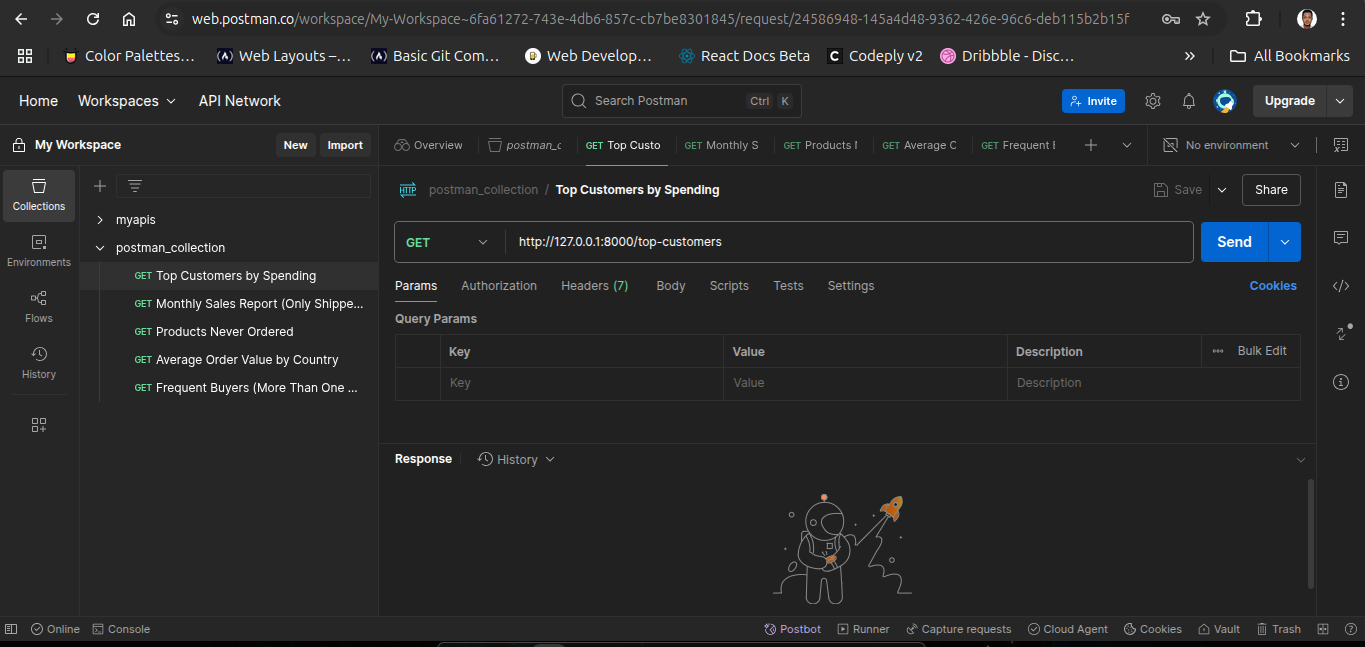
\includegraphics[width=0.9\textwidth]{screenshots/postman_api_docs.png}
\caption{Postman API Documentation}
\end{figure}

\section{Results and Screenshots}
Below are results from SQL queries and API responses.

\begin{figure}[H]
\centering
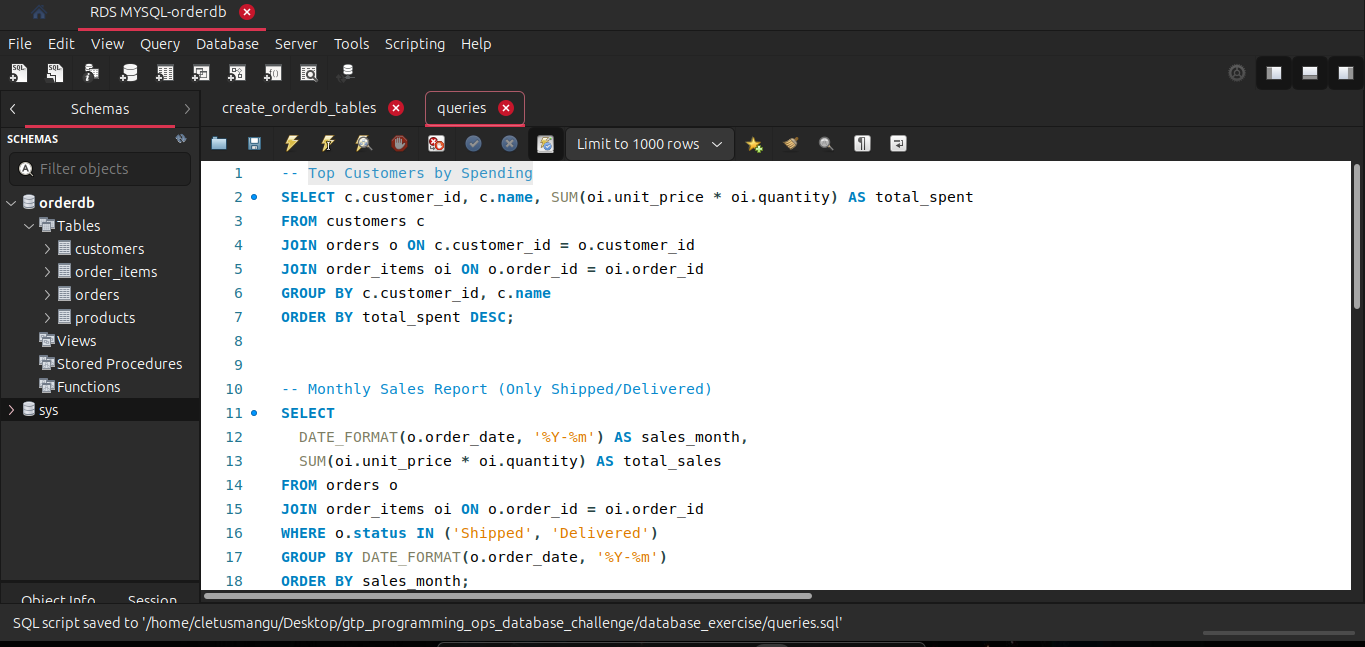
\includegraphics[width=0.9\textwidth]{screenshots/workbench_queries.png}
\caption{SQL Query Results in MySQL Workbench}
\end{figure}

\begin{figure}[H]
\centering
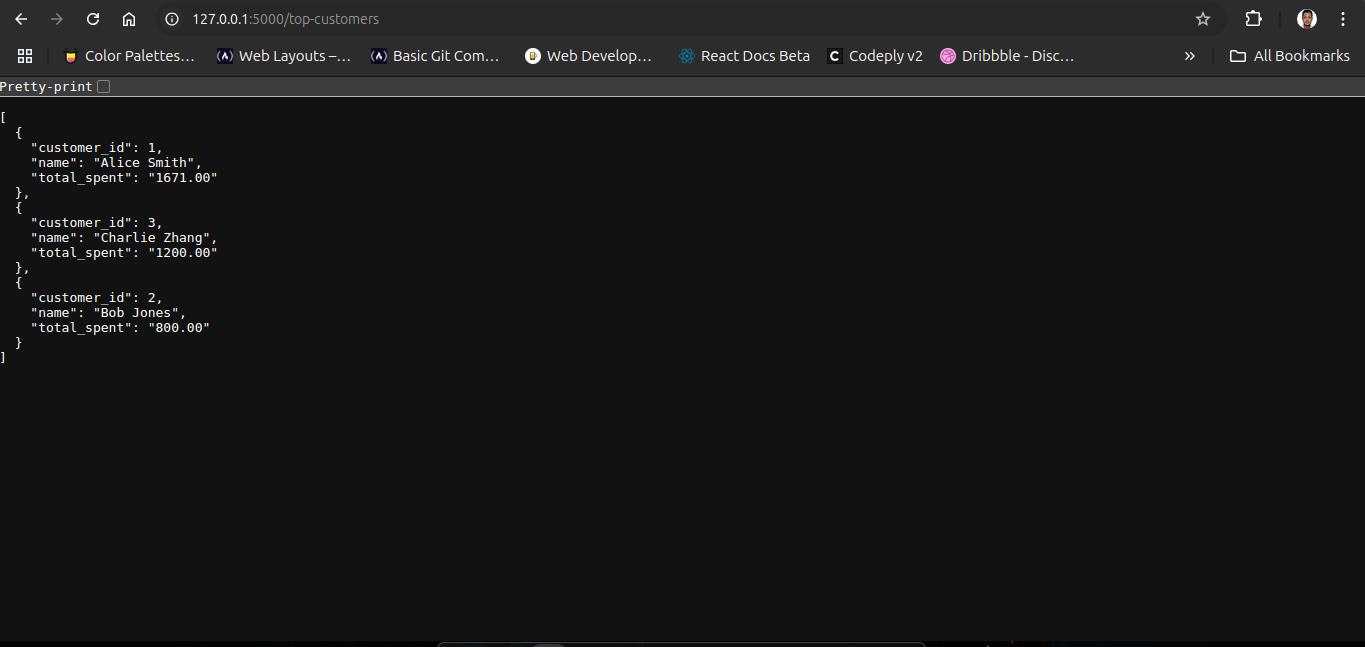
\includegraphics[width=0.9\textwidth]{screenshots/flask_response.png}
\caption{Flask API Response}
\end{figure}

\begin{figure}[H]
\centering
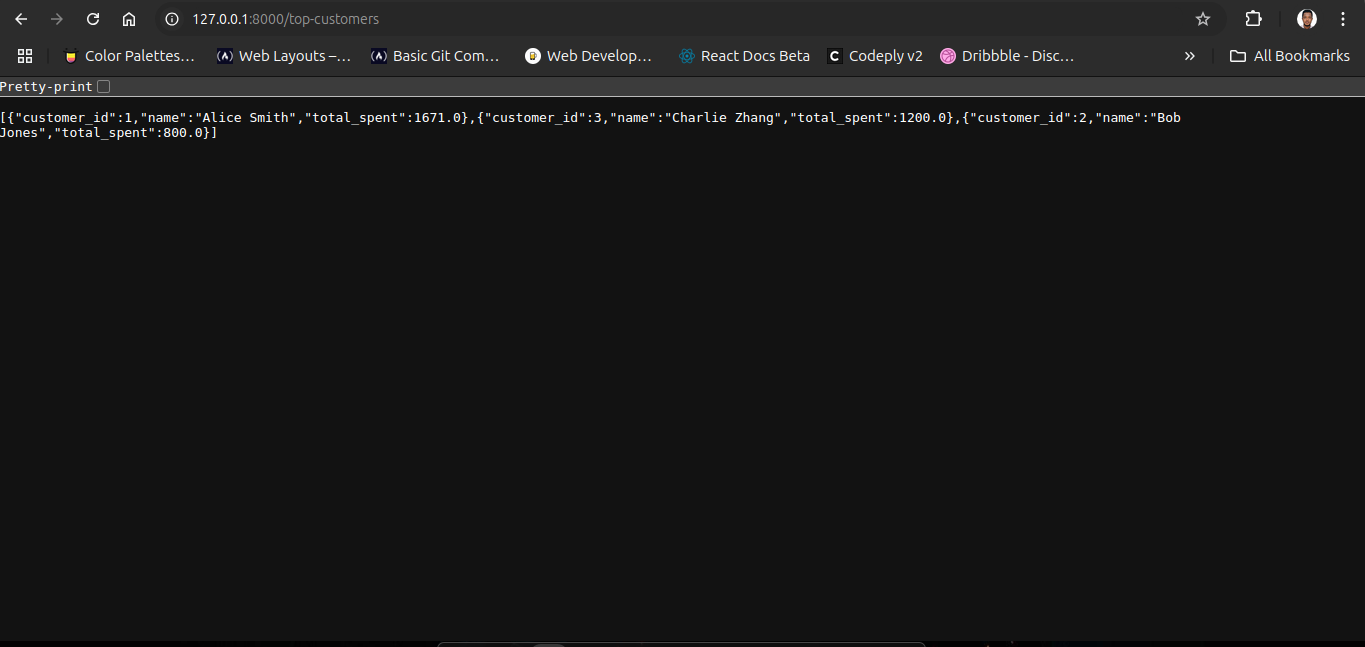
\includegraphics[width=0.9\textwidth]{screenshots/fastapi_response.png}
\caption{FastAPI Swagger UI Response}
\end{figure}

\section{Project Structure}
\begin{lstlisting}
.
├── flask_api/
│   └── app.py
├── fastapi_api/
│   └── main.py
├── postman_collection.json
├── queries.sql
├── screenshots/
│   ├── workbench_queries.png
│   ├── flask_response.png
│   ├── fastapi_response.png
│   └── postman_api_docs.png
└── README.md
\end{lstlisting}

\section{Conclusion}
This project showcases an end-to-end deployment of analytics using AWS RDS and Python APIs. It covers cloud databases, SQL analysis, REST APIs, and API documentation. This comprehensive stack is suitable for real-world reporting systems and developer portfolios.

\section{References}
\begin{itemize}
    \item AWS RDS Documentation: \url{https://docs.aws.amazon.com/rds/}
    \item Flask Documentation: \url{https://flask.palletsprojects.com/}
    \item FastAPI Documentation: \url{https://fastapi.tiangolo.com/}
    \item Postman: \url{https://www.postman.com/}
\end{itemize}

\end{document}
